% flashcards-title: Constant-velocity graph family
% flashcards-desc: Position rises linearly, velocity is a horizontal positive line, and acceleration is a horizontal line at zero over the same time interval.
\documentclass[border=7pt]{standalone}
\def\pgfsysdriver{pgfsys-dvisvgm.def}
\usepackage{tikz}
\usetikzlibrary{arrows.meta,positioning,shapes.geometric}
\definecolor{mechInk}{HTML}{172033}
\definecolor{mechBlue}{HTML}{155EEF}
\definecolor{mechOrange}{HTML}{B54708}
\definecolor{mechPale}{HTML}{E8F0FF}
\definecolor{mechGray}{HTML}{667085}
\definecolor{mechLight}{HTML}{D0D5DD}
\tikzset{
  every picture/.style={font=\sffamily\large, text=mechInk},
  mech box/.style={draw=mechInk, line width=1.2pt, rounded corners=4pt,
    fill=white, align=center, minimum height=14mm, inner xsep=5mm},
  mech primary/.style={draw=mechBlue, line width=2.2pt},
  mech secondary/.style={draw=mechOrange, line width=2.2pt, dashed},
  mech guide/.style={draw=mechGray, line width=0.9pt, dashed},
  mech arrow/.style={-{Stealth[length=3.2mm,width=2.4mm]},
    draw=mechInk, line width=1.4pt, line cap=butt},
  mech axis/.style={draw=mechInk, line width=1.2pt},
  mech tick/.style={draw=mechInk, line width=1pt}
}

\begin{document}
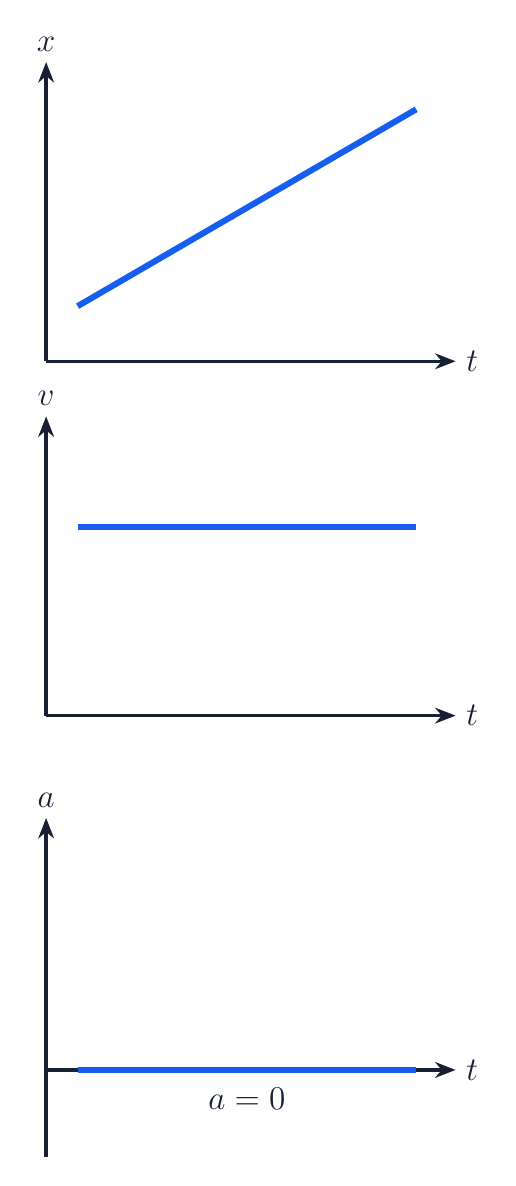
\begin{tikzpicture}[x=1cm,y=1cm]
  \begin{scope}[shift={(0,9)}]
    \draw[mech axis,-{Stealth[length=2.6mm,width=2mm]}] (0,0) -- (5.2,0) node[right] {\(t\)};
    \draw[mech axis,-{Stealth[length=2.6mm,width=2mm]}] (0,0) -- (0,3.8) node[above] {\(x\)};
    \draw[mech primary] (0.4,0.7) -- (4.7,3.2);
  \end{scope}
  \begin{scope}[shift={(0,4.5)}]
    \draw[mech axis,-{Stealth[length=2.6mm,width=2mm]}] (0,0) -- (5.2,0) node[right] {\(t\)};
    \draw[mech axis,-{Stealth[length=2.6mm,width=2mm]}] (0,0) -- (0,3.8) node[above] {\(v\)};
    \draw[mech primary] (0.4,2.4) -- (4.7,2.4);
  \end{scope}
  \begin{scope}
    \draw[mech axis,-{Stealth[length=2.6mm,width=2mm]}] (0,0) -- (5.2,0) node[right] {\(t\)};
    \draw[mech axis,-{Stealth[length=2.6mm,width=2mm]}] (0,-1.1) -- (0,3.2) node[above] {\(a\)};
    \draw[mech primary] (0.4,0) -- (4.7,0);
    \node[below=3pt] at (2.55,0) {\(a=0\)};
  \end{scope}
\end{tikzpicture}
\end{document}
